\documentclass[11pt,answers]{exam}
\usepackage[margin=0.7in]{geometry}
\usepackage{amsmath,amssymb}
\usepackage{colortbl}
\usepackage{multicol}
\usepackage{tikz,pgfplots}
\usepackage{soul}
\usepackage{circledsteps}

\newcommand{\blank}[1]{\underline{\hspace*{#1}}}
\newcommand{\ds}{\displaystyle}
\newcommand{\mymod}{~\mathrm{mod}~}


\begin{document}
\pagestyle{empty}
\graphicspath{{/home/brian/Dropbox/HSC/Spring16/Math111/}}

\subsection*{Midterm 1 Review Solutions \hfill Math \& Society}

\textit{The following problems are similar to ones you might see on the midterm exam. There is a also a list of terms \& facts you should memorize on the last page.}

\begin{questions}

\question Consider the following election. 
\begin{center}
\begin{tabular}{lcccccc}
\rowcolor{gray!30} & \multicolumn{6}{c}{\textbf{Number of Voters}} \\
\rowcolor{gray!30}  & \textbf{5} & \textbf{3} & \textbf{5} & \textbf{3} & \textbf{2} & \textbf{3} \\
Candidate A & 1st & 1st & 4th & 5th & 4th & 3rd \\ \hline 
Candidate B & 2nd & 3rd & 5th & 3rd & 3rd & 1st \\ \hline 
Candidate C & 4th & 2nd & 3rd & 1st & 1st & 5th \\ \hline 
Candidate D & 3rd & 4th & 1st & 2nd & 2nd & 4th \\ \hline 
Candidate E & 5th & 5th & 2nd & 4th & 5th & 2nd \\ \hline
\end{tabular}
\end{center}

\begin{parts}
\part Which candidate would win using the plurality method?
\begin{solution}
Candidate A
\end{solution}
\vfill
\part Which candidate would be the first eliminated in instant run-off voting?
\begin{solution}
Candidate E
\end{solution}
\vfill
\part Which candidate would win using IRV? 
\begin{solution}
Candidate A
\end{solution}
\vfill
\part Which candidate would win using IRV if Candidate D quits the election before any votes are cast?  
\begin{solution}
Candidate E
\end{solution}
\vfill
\part The fact that candidate D withdrawing from the election can change the winner means that instant run-off voting can violate one of the fairness criteria.  Which one?  
\begin{solution}
Candidate D is a spoiler candidate, so this violates the no spoilers criterion.
\end{solution}
\vfill
\end{parts}


\question Consider the weighted voting system [6:4,2,1].
\begin{parts}
\part Are any of the players dummies?  If so, which one(s)?
\begin{solution}
Yes, player C is a dummy.  
\end{solution}
\vfill
\part Do any players have veto power?  If so, which ones(s)?
\begin{solution}
Yes, both players A and B have veto power. 
\end{solution}
\vfill

\part What is the Banzhaf power index for each player?
\begin{solution}
A and B both have 50\% of the power, C has 0\% of the power. 
\end{solution}
\vfill
\end{parts}

\newpage
\question Consider the weighted voting system [7:5,3,1,1].
\begin{parts}
\part List all winning coalitions and circle the critical players in each winning coalition.
\begin{solution}
\begin{center}
\begin{tabular}{c|c|c}
2 Player & 3 Player & 4 Player \\ \hline
$\Circled{A}+\Circled{B}$ & $\Circled{A}+\Circled{B}+C$ & $\Circled{A}+B+C+D$ \\ 
~ & $\Circled{A}+\Circled{B}+D$ & ~ \\
~ & $\Circled{A}+\Circled{C}+\Circled{D}$ & ~ 
\end{tabular}
\end{center}
\end{solution}
\vfill
\vfill
\part Suppose that player $A$ sells one of her votes to player $B$, resulting in a new weighted voting system [7:4,4,1,1]. List all winning coalitions and circle the critical players in each with this new system.
\begin{solution}
\begin{center}
\begin{tabular}{c|c|c}
2 Player & 3 Player & 4 Player \\ \hline
$\Circled{A}+\Circled{B}$ & $\Circled{A}+\Circled{B}+C$ & $\Circled{A}+\Circled{B}+C+D$ \\ 
~ & $\Circled{A}+\Circled{B}+D$ & ~ \\
\end{tabular}
\end{center}
\end{solution}
\vfill
\vfill
\part What is paradoxical about the effect of $A$ selling a vote to $B$?  Write a one sentence explanation.
\begin{solution}
This causes C \& D to become dummies even though they don't lose any votes.  
\end{solution}
\vfill
\end{parts}

\question Let [$x$: 4, 3, 2, 1] be a weighted voting system with a vote threshold that has not be set yet. 
\begin{parts}
\part Is it possible to set $x$ low enough so that player $A$ (with 4 votes) is a dictator? 
\begin{solution}
No, in order for A to be a dictator, $x$ would have to be 4, but you can't set the vote threshold below 6.  If it is 5 or lower, then you could have opposite motions both pass.  
\end{solution}
\vfill
\part Is it possible to set $x$ so that every player except $D$ (with 1 vote) has veto power?  
\begin{solution}
Yes, if $x = 9$, then any winning coalition must include A, B, and C, so they each have veto power.  
\end{solution}
\vfill
\end{parts}

\question Suppose that a business has four partners (A, B, C, and D).  Each partner has one vote and decisions are made by majority rule, except when there is a tie.  If there is a tie, then since A is the senior partner, their vote is the tie breaker.  
\begin{parts}
\part Find all of the winning coalitions and circle the critical players in each coalition.
\begin{solution}
\begin{center}
\begin{tabular}{c|c|c}
2 Player & 3 Player & 4 Player \\ \hline
$\Circled{A}+\Circled{B}$ & $\Circled{A}+B+C$ & $A+B+C+D$ \\ 
$\Circled{A}+\Circled{C}$ & $\Circled{A}+B+D$ & ~ \\
$\Circled{A}+\Circled{D}$ & $\Circled{A}+C+D$ & ~ \\
~ & $\Circled{B} + \Circled{C} + \Circled{D}$ & ~ 
\end{tabular}
\end{center}
\end{solution}
\vfill
\vfill
\part Find the Banzhaf power index for each of the four partners.
\begin{solution}
A has $\tfrac{6}{12} = \tfrac{1}{2}$ of the power, and B, C, and D each have $\tfrac{2}{12} = \tfrac{1}{6}$ of the power.
\end{solution}
\vfill
\end{parts}
\newpage

\question Suppose that an election is held with three candidates using the Borda count method.  The voter preferences are shown in the table below. 

\begin{center}
\begin{tabular}{lcccc}
\rowcolor{gray!30} & \multicolumn{4}{c}{\textbf{Number of Voters}} \\
\rowcolor{gray!30}  & \textbf{20} & \textbf{10} & \textbf{5} & \textbf{2} \\
Ava & 1st & 3rd & 3rd & 2nd \\ \hline
Bill & 2nd & 1st & 2nd & 1st \\ \hline
Callie & 3rd & 2nd & 1st & 3rd \\ \hline
\end{tabular}
\end{center}

\begin{parts}
\part How many points does each candidate get?  
\begin{solution}
Ava gets 79, Bill gets 86, and Callie gets 57 points.
\end{solution}
\vfill
\part Show that Ava would get more points than Bill if Callie dropped out of the election.  
\begin{solution}
If Callie dropped out, then 17 voters would pick Bill first and 20 would pick Ava first.  So Ava would get more points (57) than Bill (54).
\end{solution}
\vfill
\part Show that Ava would also beat Callie in a head-to-head vote. 
\begin{solution}
Ava would get 22 votes against Callie's 15 votes in a head-to-head vote.
\end{solution}
\vfill
\part Parts (b) \& (c) show that Borda count can fail two different fairness criteria.  Which two?  
\begin{solution}
Ava is a Condorcet candidate, but she loses to Bill when three candidates run.  Callie is also a spoiler, since Ava would have won if Callie hadn't run.  So this election fails both the Condorcet and no spoilers criteria. 
\end{solution}
\vfill
\end{parts}

\question Use the logarithmic scale below and a piece of paper to measure and mark the exact location of the following numbers. Be sure to clearly indicate which mark goes with which number.  
\bigskip

\begin{center}
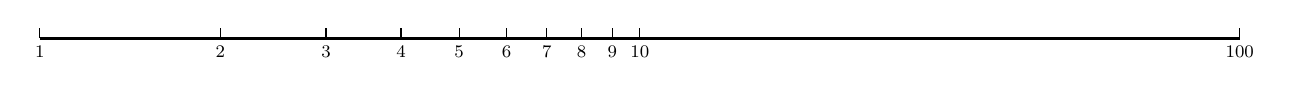
\begin{tikzpicture}
\draw[very thick] (0,0) -- (6in,0);
\foreach \i in {1,2,3,4,5,6,7,8,9,10,100} {
	\pgfmathparse{3*(ln(\i)/ln(10)) };
	\draw (\pgfmathresult in,0) node[below,scale=0.8] {\footnotesize \i}  -- +(0,0.05in);
}
\end{tikzpicture}
\end{center}
\bigskip

\begin{parts}
\part 50

\part 1.5 (Hint: what fraction is 1.5 the same as?)

\part $\tfrac{100}{7}$

\end{parts}

\begin{solution}
\begin{center}
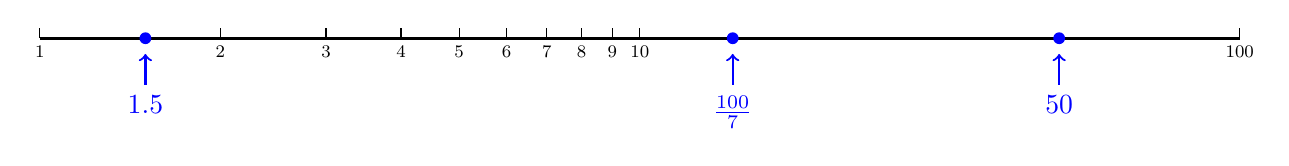
\begin{tikzpicture}
\draw[very thick] (0,0) -- (6in,0);
\foreach \i in {1,2,3,4,5,6,7,8,9,10,100} {
	\pgfmathparse{3*(ln(\i)/ln(10)) };
	\draw (\pgfmathresult in,0) node[below,scale=0.8] {\footnotesize \i}  -- +(0,0.05in);
}
\draw[<-,thick, blue] (0.5283 in, -0.2) -- +(0,-0.4) node[below] {1.5};
\fill[blue] (0.5283 in, 0) circle (0.075);
\draw[<-,thick, blue] (5.097 in, -0.2) -- +(0,-0.4) node[below] {50};
\fill[blue] (5.097 in, 0) circle (0.075);
\draw[<-,thick, blue] (3.4647 in, -0.2) -- +(0,-0.4) node[below] {$\tfrac{100}{7}$};
\fill[blue] (3.4647 in, 0) circle (0.075);

\end{tikzpicture}
\end{center}

\end{solution}
\vfill
\newpage

\question According to the rule of 70, how long would it take for a debt that earns 14\% interest every year to double if you don't pay any money back?  
\begin{solution}
About 5 years.
\end{solution}
\vfill

\question Suppose that I invest \$400 in the stock market. If my investments grow 50\% the first year, then decline 30\% the next, and then decline 20\% in the third year, how much money will I have after three years?
\begin{solution}
$$400(1.50)(0.70)(0.8) = \$336.$$
\end{solution}
\vfill

\question Bob invests \$1,000 in a mutual fund that grows at 3\% per year.  Carol invests \$1,000 in a CD that grows 2\% per year.  
\begin{parts}
\part How much money do Bob and Carol each have after 10 years?  
\begin{solution} 
Bob has $1{,}000(1.03^{10}) = \$1{,}343.92$ and Carol has $1{,}000(1.02^{10}) = \$1{,}218.99.$
\end{solution}
\vfill
\part Relative to Carol, how much more money does Bob have?  Express your answer by completing the following sentence:
\begin{center}
Bob has \underline{\hspace*{0.5in}}\% more money than Carol.
\end{center}
\begin{solution}
Bob has 1.10 times more money than Carol, so he has \underline{~10\%~} more money than Carol.
\end{solution}
\end{parts}
\vfill

\question The age of a tree is roughly proportional to the diameter of its trunk. Suppose that you know that one red maple tree has a trunk diameter of 10 inches and is 45 years old. A second red maple has a trunk diameter of 16 inches. Set up and solve a proportion equation to estimate how old that second tree is.
\begin{solution}
Let $x$ be the age of the second tree. Then
$$\dfrac{45}{10} = \dfrac{x}{16}$$
so $x = \dfrac{(16)(45)}{10} = 72$ years old.  
\end{solution}
\vfill

\newpage
\question Convert each of the following percentage changes into a growth factor. 
\begin{parts}
\part 36\% increase.
\begin{solution}
Same as multiplying by a factor of 1.36.  
\end{solution}
\vfill

\part 60\% decrease.
\begin{solution}
Same as multiplying by a factor of 0.40.  
\end{solution}
\vfill

\part 200\% increase.
\begin{solution}
Same as multiplying by a factor of 3.  
\end{solution}
\vfill

\end{parts}

\question For each of the following patterns, determine whether it is an arithmetic or geometric sequence. If it is arithmetic, find the common step size.  If it is geometric find the common ratio. 
\begin{parts}
\part $5, ~ 25, ~ 125, ~ 625, ~ \ldots$
\begin{solution}
Geometric.  The common ratio is $5$. 
\end{solution}
\vfill

\part $320, ~ 280, ~ 240, ~ 200, ~ 160, ~ \ldots$
\begin{solution}
Arithmetic.  The common step size is $-40$. 
\end{solution}
\vfill
\part $1.05, ~ 1.10, ~ 1.15, ~ 1.20, ~ 1.25, ~ \ldots$
\begin{solution}
Arithmetic. The common step size is $0.05$
\end{solution}
\vfill
\end{parts}

\question Use factor-label method to solve the following problem.  Clearly show each conversion factor that you used. 
Suppose a swimming pool contains 10,000 cubic feet of water.  A cubic foot of water is approximately 7.5 gallons, and a gallon weighs approximately 8.344 lbs. How much does the water in the pool weigh?  
\begin{solution}
$$10{,}000 \text{ cu. ft.} \left( \frac{7.5 \text{ gallons}}{1 \text{ cu. ft.}} \right) \left( \frac{8.344 \text{ lbs.}}{1 \text{ gallon}} \right)  = 625{,}800 \text{ lbs.}$$
\end{solution}
\vfill
\vfill


\question Write the number $(3 \text{ trillion})^3$ in scientific notation.
\begin{solution}
$$(3 \times 10^{12})^3 = 27.0 \times 10^{36} = 2.7 \times 10^{37}.$$
\end{solution}
\vfill
\end{questions}

\newpage
\subsection*{Midterm 1 Study Guide \hfill Math \& Society}

\subsubsection*{Voting Theory}

You should know how to find the winner of an election using the following methods: \textbf{plurality}, \textbf{Borda count}, \textbf{instant run-off}, and \textbf{approval voting}.  You should be able to identify \textbf{Condorcet} and \textbf{spoiler candidates}.  You should know the following fairness criteria: \textbf{no spoilers}, \textbf{Condorcet}, and \textbf{monotonicity}. Memorize this table showing which methods always satisfy which fairness criteria.

\begin{center}
\begin{tabular}{l|ccc} 
~ & Condorcet & Monotonicity & No Spoiler  \\ \hline
Plurality method & No & Yes & No \\
Instant run-off voting & No & No & No \\
Borda count & No & Yes & No \\
Approval voting & No & Yes & Yes \\ 
\end{tabular}
\end{center}

Finally, you should know about \textbf{Arrow's impossibility theorem} which says that no voting method can have always satisfy both the no spoilers and Condorcet criterion.  

\subsubsection*{Weighted Voting Theory}

Be sure you can find the \textbf{winning coalitions}, \textbf{critical players}, and \textbf{Banzhaf power index} for a weighted voting system.  You should also know the following terms: \textbf{dictator}, \textbf{dummy}, and \textbf{veto power}. 

\subsubsection*{Multiplicative Reasoning}

Be able to set up and solve \textbf{proportion equations}.  Be able to identify the \textbf{units} of numbers and know that a \textbf{factor} is a number or expression that is being multiplied or divided.  You should be comfortable using \textbf{conversion factors} to solve problems using \textbf{factor-label method}.  

Know the difference between \textbf{arithmetic} and \textbf{geometric sequences} of numbers.  Understand how to multiply and divide numbers on a \textbf{logarithmic scale} and be familiar with \textbf{orders of magnitude} and \textbf{scientific notation} including the number words \textbf{million}, \textbf{billion}, \textbf{trillion}, and the metric prefixes \textbf{milli}, \textbf{centi} and \textbf{kilo}.  

You will need to be able to convert from \textbf{growth factors} to \textbf{percent change} and vice versa. You should also be able to calculate \textbf{compound interest} and know the \textbf{rule of 70}.   

\end{document}
